\hypertarget{Options_8cpp}{\section{Options.\+cpp File Reference}
\label{Options_8cpp}\index{Options.\+cpp@{Options.\+cpp}}
}


Implementation of classes to represent an option an a put option.  


{\ttfamily \#include $<$cmath$>$}\\*
{\ttfamily \#include \char`\"{}Options.\+h\char`\"{}}\\*
Include dependency graph for Options.\+cpp\+:\nopagebreak
\begin{figure}[H]
\begin{center}
\leavevmode
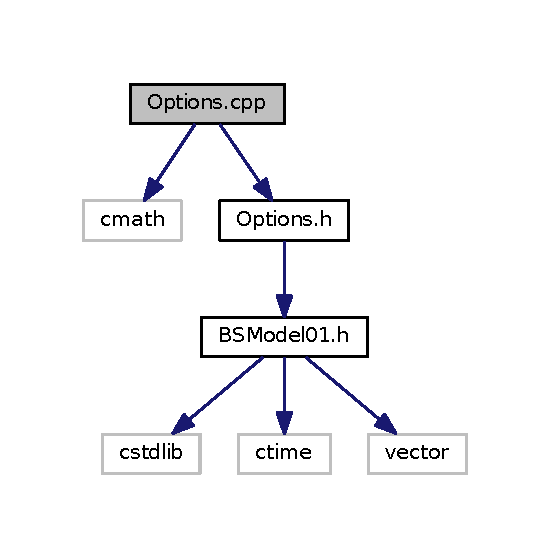
\includegraphics[width=264pt]{Options_8cpp__incl}
\end{center}
\end{figure}


\subsection{Detailed Description}
We write out classes which will be used to store the coefficients and boundary conditions in order to price options under the Black--Scholes equation. We represent an option as an abstract class. Its methods will the overridden by the put option class

\begin{DoxyWarning}{Warning}
This code is also listed and fully explained in the book $\ast$$\ast$\+Numerical Methods in Finance with C++$\ast$$\ast$ by Maciej Capiński and Tomasz Zastawniak, published in September 2012.
\end{DoxyWarning}
\begin{DoxyAuthor}{Author}
\+: Eduardo J. Sanchez (ejspeiro) -\/ ejspeiro at gmail dot com 
\end{DoxyAuthor}


Definition in file \hyperlink{Options_8cpp_source}{Options.\+cpp}.

